%% This is file `elsarticle-template-1-num.tex',
%%
%% Copyright 2009 Elsevier Ltd
%%
%% This file is part of the 'Elsarticle Bundle'.
%% ---------------------------------------------
%%
%% It may be distributed under the conditions of the LaTeX Project Public
%% License, either version 1.2 of this license or (at your option) any
%% later version.  The latest version of this license is in
%%    http://www.latex-project.org/lppl.txt
%% and version 1.2 or later is part of all distributions of LaTeX
%% version 1999/12/01 or later.
%%
%% The list of all files belonging to the 'Elsarticle Bundle' is
%% given in the file `manifest.txt'.
%%
%% Template article for Elsevier's document class `elsarticle'
%% with numbered style bibliographic references
%%
%% $Id: elsarticle-template-1-num.tex 149 2009-10-08 05:01:15Z rishi $
%% $URL: http://lenova.river-valley.com/svn/elsbst/trunk/elsarticle-template-1-num.tex $
%%
\documentclass[finalreport,12pt]{elsarticle}


% % Following code is to eliminte the "preprint submitted to journal name" footer. 
\makeatletter
\def\ps@pprintTitle{%
 \let\@oddhead\@empty
 \let\@evenhead\@empty
 \def\@oddfoot{\centerline{\thepage}}%
 \let\@evenfoot\@oddfoot}
\makeatother

%% Use the option review to obtain double line spacing
%% \documentclass[preprint,review,12pt]{elsarticle}

%% Use the options 1p,twocolumn; 3p; 3p,twocolumn; 5p; or 5p,twocolumn
%% for a journal layout:
%% \documentclass[final,1p,times]{elsarticle}
%% \documentclass[final,1p,times,twocolumn]{elsarticle}
%% \documentclass[final,3p,times]{elsarticle}
%% \documentclass[final,3p,times,twocolumn]{elsarticle}
%% \documentclass[final,5p,times]{elsarticle}
%% \documentclass[final,5p,times,twocolumn]{elsarticle}

%% if you use PostScript figures in your article
%% use the graphics package for simple commands
%% \usepackage{graphics}
%% or use the graphicx package for more complicated commands
%% \usepackage{graphicx}
%% or use the epsfig package if you prefer to use the old commands
%% \usepackage{epsfig}

%% The amssymb package provides various useful mathematical symbols
\usepackage{amssymb}
%% The amsthm package provides extended theorem environments
%% \usepackage{amsthm}

%% The lineno packages adds line numbers. Start line numbering with
%% \begin{linenumbers}, end it with \end{linenumbers}. Or switch it on
%% for the whole article with \linenumbers after \end{frontmatter}.
\usepackage{lineno}
\usepackage{capt-of}
\usepackage{pgfplots}

%% natbib.sty is loaded by default. However, natbib options can be
%% provided with \biboptions{...} command. Following options are
%% valid:

%%   round  -  round parentheses are used (default)
%%   square -  square brackets are used   [option]
%%   curly  -  curly braces are used      {option}
%%   angle  -  angle brackets are used    <option>
%%   semicolon  -  multiple citations separated by semi-colon
%%   colon  - same as semicolon, an earlier confusion
%%   comma  -  separated by comma
%%   numbers-  selects numerical citations
%%   super  -  numerical citations as superscripts
%%   sort   -  sorts multiple citations according to order in ref. list
%%   sort&compress   -  like sort, but also compresses numerical citations
%%   compress - compresses without sorting
%%
%% \biboptions{comma,round}

% \biboptions{}


\journal{A Journal}

\begin{document}

\begin{frontmatter}

%% Title, authors and addresses

%% use the tnoteref command within \title for footnotes;
%% use the tnotetext command for the associated footnote;
%% use the fnref command within \author or \address for footnotes;
%% use the fntext command for the associated footnote;
%% use the corref command within \author for corresponding author footnotes;
%% use the cortext command for the associated footnote;
%% use the ead command for the email address,
%% and the form \ead[url] for the home page:
%%
%% \title{Title\tnoteref{label1}}
%% \tnotetext[label1]{}
%% \author{Name\corref{cor1}\fnref{label2}}
%% \ead{email address}
%% \ead[url]{home page}
%% \fntext[label2]{}
%% \cortext[cor1]{}
%% \address{Address\fnref{label3}}
%% \fntext[label3]{}

\title{Comparing Concurrent AVL Trees}

%% use optional labels to link authors explicitly to addresses:
%% \author[label1,label2]{<author name>}
%% \address[label1]{<address>}
%% \address[label2]{<address>}

\author{Nick Carlson, Paul Iwatake}

% %\address{California, United States}

\begin{abstract}
%% Text of abstract
Summary and discussion of the implementation of lock and lockfree variants of AVL trees in two different programming languages, and analysis comparing its performance with related tree implementations. 
\end{abstract}

\begin{keyword}
AVL Tree \sep Concurrency 
%% keywords here, in the form: keyword \sep keyword

%% MSC codes here, in the form: \MSC code \sep code
%% or \MSC[2008] code \sep code (2000 is the default)

\end{keyword}

\end{frontmatter}

%%
%% Start line numbering here if you want
%%
%%\linenumbers

%% main text
\section{Introduction}
\label{S:1}

% %\cite{Smith:2012qr} \cite{Smith:2013jd} 

For our project, we set out to compare implementations of balanced tree data structures, or AVL trees. Initially, we wanted to compare an implementation created in an imperative language, versus a functional language. We planned to use Haskell, C++, Google Go, and Scala, but had to scale down to using two imperative languages, C++ and Go, instead, due to time constraints. 

We had wanted to use functional languages due to their ease of paralellization, as they can be easier to prove correctness with, automatically put in parallel with some tools, and other characteristics that cater well to concurrency.

	Various research has been conducted involving variants of non-blocking binary search trees \cite{Bronson}, \cite{Brown}, \cite{Wicht}, but we could not find many concurrent AVL trees implementations using locks freely available, bar one \cite{Wicht}. Obviously more research has focused on non-blocking trees in the interest of speed and efficiency. We also tried to incorporate some ideas from concurrent Red-Black Trees \cite{Kim}.
	
	We did not seek to reinvent the wheel, so to speak, but to gain experience in concurrency using programming languages we were not entirely familiar with. As such, we started out with a coarse grain lock approach, then moved on to a fine grained lock, before attempting to apply non-locking implementations. 



\iffalse

\begin{itemize}
\item Bullet point one
\item Bullet point two
\end{itemize}

\begin{enumerate}
\item Numbered list item one
\item Numbered list item two
\end{enumerate}

\fi

\iffalse

\begin{table}[h]
\centering
\begin{tabular}{l l l}
\hline
\textbf{Treatments} & \textbf{Response 1} & \textbf{Response 2}\\
\hline
Treatment 1 & 0.0003262 & 0.562 \\
Treatment 2 & 0.0015681 & 0.910 \\
Treatment 3 & 0.0009271 & 0.296 \\
\hline
\end{tabular}
\caption{Table caption}
\end{table}

\fi


% %\begin{equation}
% %\label{eq:emc}
% %e = mc^2
% %\end{equation}

\section{Related Work}
\label{S:2}

Similar tree structures include the Skip List\cite{Wicht}, non-blocking trees using Compare-and-Swap (CAS) constructs\cite{Brown}, and a concurrent relaxed balance AVL tree\cite{Bronson}.

\subsection{Skip List}
The skip list is a probabilistic data structure essentially consisting of a hierarchal linked list where each node has many links, linking few nodes at the top of the hierarchy so that those nodes have "shortcut" links, and all the nodes at the bottom of the hierarchy. Nodes are assigned a level randomly at insertion time\cite{Wicht}. 

This is a popular (An implementation exists in the Java library, so that says something) quickly-searched data structure because of its simplicity to implement compared to a tree, where concurrent rebalancing can lead to significant bottlenecks\cite{Wicht}.

\subsection{Non-blocking Tree}

One implementation of a tree data structure not using locks was found using CAS primitives. It uses multiword versions of the primitives load-link (LL), store-conditional (SC), and validate (VL), just multiword versions, denoted as LLX, SCX, and VLX respectively instead. These operate on "data-records", data structures that consist of a fixed number of mutable and immutable fields. 

LLX is used to take a snapshot of a given data record, which may fail if overlapping with an SCX operation. SCX, as its name might imply, tries to atomically change a value of a mutable member of a data record, then make a data record "finalized" so that further LLX returns that status instead of a snapshot. Processes involved SCX and VLX must do an LLX that succeeds and produces a valid snapshot before they can proceed. VLX can then be used by the same process to see that the data record(s) have not changed since the last LLX call by the same process. In this way it obtains a snapshot of data-records, since it may also operate on a set. 

Using these primitives, it is possible to implement a chromatic tree that is provably correct, using a try-fail-retry strategy, that marks violations in the tree for cleanup later\cite{Brown}. 


\subsection{Relaxed Balanced AVL Tree}

Yet another closely related structure is the relaxed balanced AVL tree. It is an optimistic structure, implemented in such a way that reads and writes have specific atomic regions that can be known ahead of time. To do this, it utilizes hand-over-hand locking, mutations that rebalance on their own, and deletions that sometimes leave behind a routing node\cite{Bronson}. A variant of this uses a linearizeable 'clone' operation to help enforce consistency. 

An idea this uses that is worth explaining is that of the external tree. This is in contrast with an internal tree, which is the usual AVL tree. In an external tree, all actual values in the tree are stored on leaves. Any non-leaf (internal) node is a 'routing' node, to aid in traversal only. This introduces some overhead with the extra nodes and the traversal of them, but it allows for much less complicated deletes, which can incur serious rebalancing issues. The relaxed balanced AVL tree uses a partially external tree structure\cite{Bronson}. 

\section{Performance}
\label{S:3}
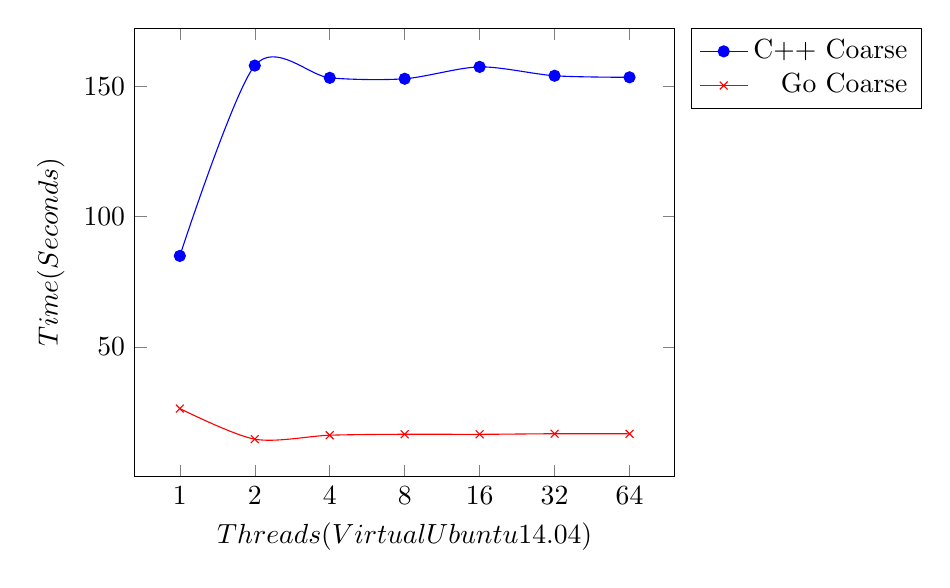
\begin{tikzpicture}

    \begin{axis}[
    	%xmin = 0,
    	xtick={1,2,3,4,5,6,7},
    	xticklabels = {1,2,4,8,16,32,64},
        xlabel=$Threads(Virtual Ubuntu 14.04)$,
        ylabel=$Time(Seconds)$,
        %enlargelimits=false
        legend style={
        cells={anchor=east},
        legend pos=outer north east,
        }
        ]
    \addplot[smooth,mark=*,blue] plot coordinates {
        (1,84.95)
        (2,157.95)
        (3,153.25)
        (4,152.9)
        (5, 157.45)
        (6, 154.05)
        (7, 153.45)
    };
    \addlegendentry{C++ Coarse}

    \addplot[smooth,color=red,mark=x]
        plot coordinates {
            (1,26.4080987)
            (2,14.6625888)
            (3,16.1832054)
            (4,16.5506131)
            (5, 16.5262005)
            (6, 16.7489493)
            (7, 16.7239604)
        };
    \addlegendentry{Go Coarse}
    \end{axis}
    %\caption{stuff}

    \end{tikzpicture}
    

   
   
   
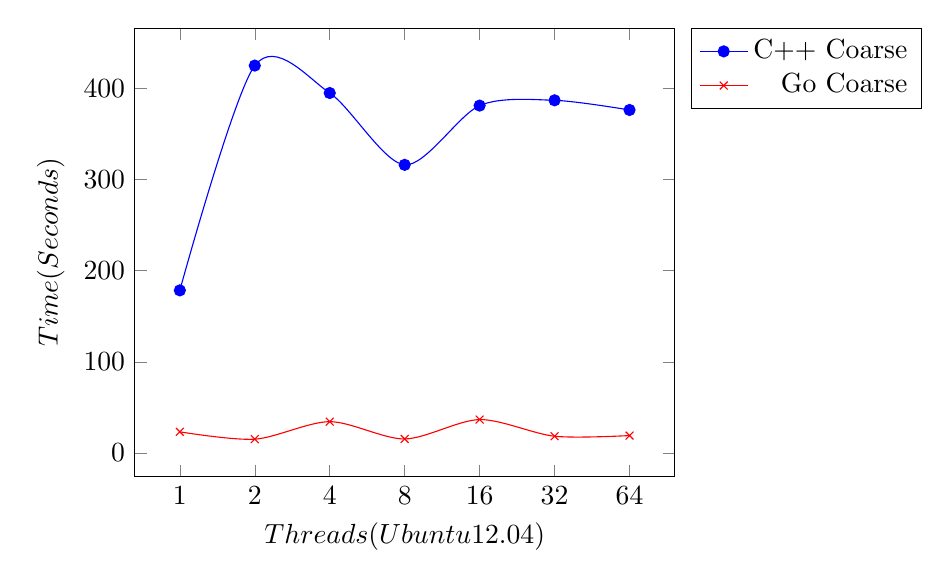
\begin{tikzpicture}

    \begin{axis}[
    	%xmin = 0,
    	xtick={1,2,3,4,5,6,7},
    	xticklabels = {1,2,4,8,16,32,64},
        xlabel=$Threads(Ubuntu 12.04)$,
        ylabel=$Time(Seconds)$,
        %enlargelimits=false
        legend style={
        cells={anchor=east},
        legend pos=outer north east,
        }
        ]
    \addplot[smooth,mark=*,blue] plot coordinates {
        (1,178.5)
        (2,425.1)
        (3,395)
        (4, 316.2)
        (5, 381.2)
        (6,  387)
        (7, 376.4)
    };
    \addlegendentry{C++ Coarse}

    \addplot[smooth,color=red,mark=x]
        plot coordinates {
            (1,23.2991678)
            (2,15.2396587)
            (3,34.463666)
            (4,15.4983169)
            (5,  36.7421332)
            (6, 18.4732514)
            (7, 19.2107438)
        };
    \addlegendentry{Go Coarse}
    \end{axis}
    %\caption{stuff}

    \end{tikzpicture}



%\newline
Testing was done on a virtual machine Ubuntu 64-bit 14.04 Linux system (2-Core 3.5 GHz processor) in order to utilize pthreads, and on a regular Ubuntu 32-bit 12.04 Linux system (2-Core 2.53 GHz processor). Testing procedure was to start with a tree of size 1, and to undertake an average workload doing 100 million operations, inserting possible values from 0 to 1 billion, with average workload defined as 90 \% contains, 9 \% insert, and 1 \% delete. Tests were conducted 5 or more times for each number of threads, then averaged. Performance was compared by calculating runtime in seconds (So fewer seconds means better performance).

12.04 Ubuntu testing may have a minor descrepancy in the Go data, since the tests were done discontinuously, so there is apparentally a spike (notable at 4 and 16 threads) in runtime due to initialization overhead for the program. But, this is still not enough to explain away the huge difference in performance between Go and C++. At times, Go seems to outperform C++ by more than a factor of ten. This is a huge difference. Possible reasons for this are that C++ pthreads are starting to show their age, or that Go's goroutines act significantly differently than regular threads. It is also quite possible our implementation for Go was flawed in some way, but this is not clear. 


We found two projects kind enough to make their code freely available on GitHub, so it would make comparison testing quite simple, given additional time. 



\section{Our Approach}
\label{S:4}

Most of the ideas for the approach come from concurrent red-black trees\cite{Kim}. It uses a variable to keep track of the version of the nodes. If the version changes while the node is trying to traverse, that means that the nodes' pointers have changed and the operation would need to start again from the top. The version of the node updates whenever there is an add performed or a rotation performed. 

So for contains operations, it would never have to obtain a lock, merely store a local copy of the node at the beginning of its call and check the version of the node as it tries to advance. Insert and Delete will both still need to lock to function correctly. Now to handle the rotate function, every node maintained a parent pointer that it would use to “climb-up” the tree. As the nodes rotate, they lock, their versions update, and a Boolean is set to marked. This Boolean allows inserting and deleting threads to know that there is a rotation going on and to return to the top of the tree and start again. 

\subsection{Difficulties In Implementation}
Other than the abandoning the functional language implementations due to time, other problems were most of the functionality of C++ that we had researched and thought would be available to us, were not. The C++ 2011 libraries such as thread and chrono were not available and alternatives such as boost did not work either. Furthermore, the research we based our tree off of required the use of Compare and Swaps, something that could not be done in C++ without making it ourselves or getting the newer libraries to work.

\section{Conclusion and Future Work}
\label{S:5}

To summarize, comparing concurrent AVL trees in different languages proved an interesting task. In the future, it would be interesting to go back and actually finish the original comparison we sought, which was comparing functional language and imperative language AVL tree concurrency. 
%% The Appendices part is started with the command \appendix;
%% appendix sections are then done as normal sections
%% \appendix

%% \section{}
%% \label{}

%% References
%%
%% Following citation commands can be used in the body text:
%% Usage of \cite is as follows:
%%   \cite{key}          ==>>  [#]
%%   \cite[chap. 2]{key} ==>>  [#, chap. 2]
%%   \citet{key}         ==>>  Author [#]

%% References with bibTeX database:



% %\bibliographystyle{model1-num-names}
% %\bibliography{sample.bib}

%% Authors are advised to submit their bibtex database files. They are
%% requested to list a bibtex style file in the manuscript if they do
%% not want to use model1-num-names.bst.

%% References without bibTeX database:

\section*{References}
 \begin{thebibliography}{5}

% \bibitem must have the following form:
%  \bibitem{key}...


\bibitem{Bronson}
  N.G. Bronson, J. Casper, H. Chafi,  and K. Olukotun, A Practical Concurrent Binary Search Tree. \emph {PPoPP '10: Proceedings of the 15th ACM SIGPLAN Symposium on Principals and Practice of Parallel Programming}, 2010.
  
  \bibitem{Brown}
	  T. Brown, F. Ellen, and E. Ruppert,  A General Technique for Non-blocking Trees. \emph {PPoPP '14: Proceedings of the 19th ACM SIGPLAN symposium on Principles and practice of parallel programming}, 2014.
	  		  
	\bibitem{Wicht}
		B. Wicht,  Binary Trees Implementations Comparison for Multicore Programming. \emph{Switzerland HES-SO University of applied science}, 2012.
		
	\bibitem{Kim}
		J.H. Kim, H. Cameron, and P. Graham,  Lock-Free Red-Black Trees Using CAS. \emph{ Concurrency
		and Computation: Practice and Experience}, 2006.

 \end{thebibliography}



\end{document}

%%
%% End of file `elsarticle-template-1-num.tex'.
